\section{Introduction}

% Discuss:

% the problem domain, 
% The scientific  hypothesis for FRESNEL (biology, physics, technology), 
% the technology and 
% the need for the experiment. 



In \proj (\textbf{F}ield expe\textbf{R}iments for mod\textbf{E}ling,
a\textbf{S}similatio\textbf{N} and adaptiv\textbf{E}
samp\textbf{L}ing) we propose to close the
observe-assimilate-predict-sample loop in the coastal ocean. Model
skill, especially in this domain, is highly dependent on sparsely
sampled in-situ measurements and remote sensing data (when
available). Typically satellite remote-sensing data augmented by some
fixed assets such as buoys, or Lagrangian floats constitute the bulk
of the observations along with a few ship-board measurements providing
validation of the model. However few models provide assimilated
information at fine spatial scales ($\sim 100$'s of meters) relevant
to short term tactical planning.

Our objective in \proj is to demonstrate the applicability of
adaptively controlled marine robots in the aerial, surface and
underwater domains, while sampling the upper water-column \emph{'at
  the right place and time'} driven by ocean models with increasing
predictive skill. Fig. \ref{fig:block-diag} shows a conceptual view of
the proposed field experiment. In doing so, we wish to:

\begin{figure}[!b]
  \centering
  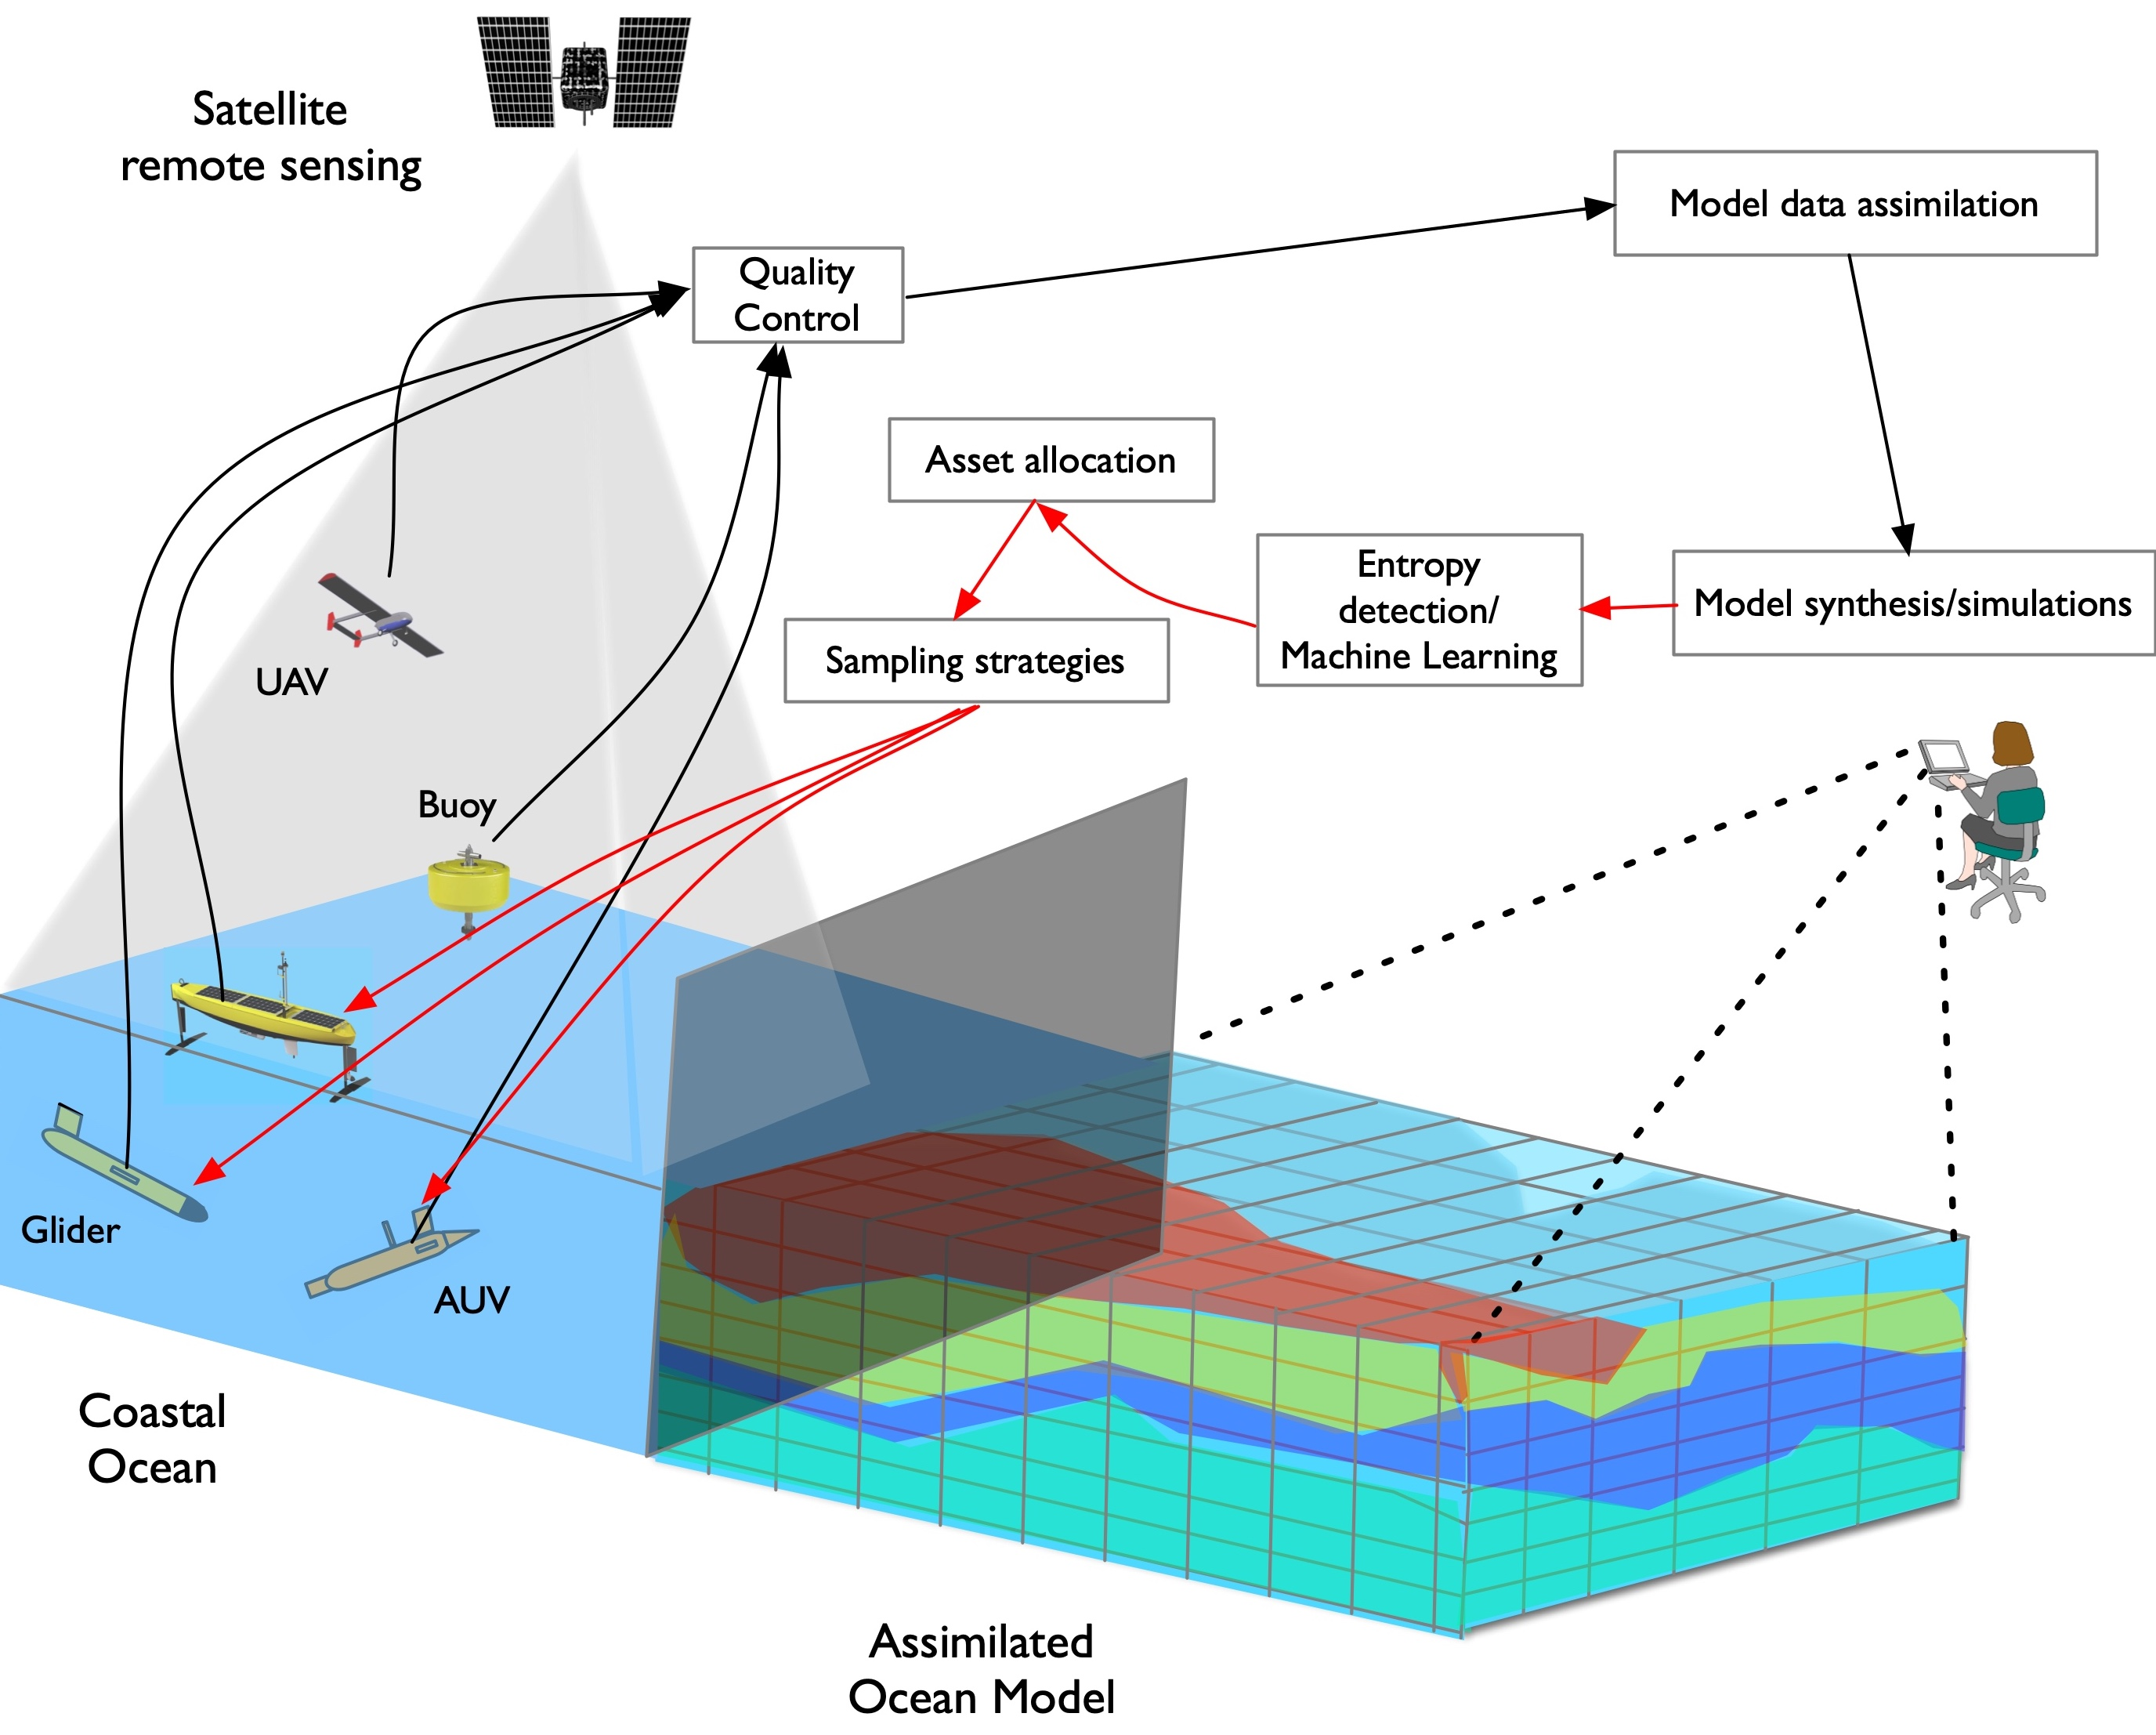
\includegraphics[scale=0.15]{fig/ensemble.jpg}
  \caption{\proj will integrate ocean models with adaptive AI-driven
    robotic vehicles in the coastal ocean, to increase model skill
    while increasing model accuracy and prediction with a tight
    control loop.}
  \label{fig:block-diag}
\end{figure}

% [noitemsep,topsep=0pt,parsep=0pt,partopsep=0pt]
\begin{enumerate}

\item Increase the predictive skill of coastal ocean models

\item Leverage the advances in Artificial Intelligence driven
  dynamic-decision making to place mobile assets in the 'right place
  at the right time'

\item Close the sense-assimilate-predict-sample loop
  
\item Advance the efforts to bring modern Machine Learning methods for
  adaptation and prediction in the advancement of our understanding of
  coastal ocean processes
  
\end{enumerate}

\begin{wrapfigure}{!h}{2.75in}
  \centering
  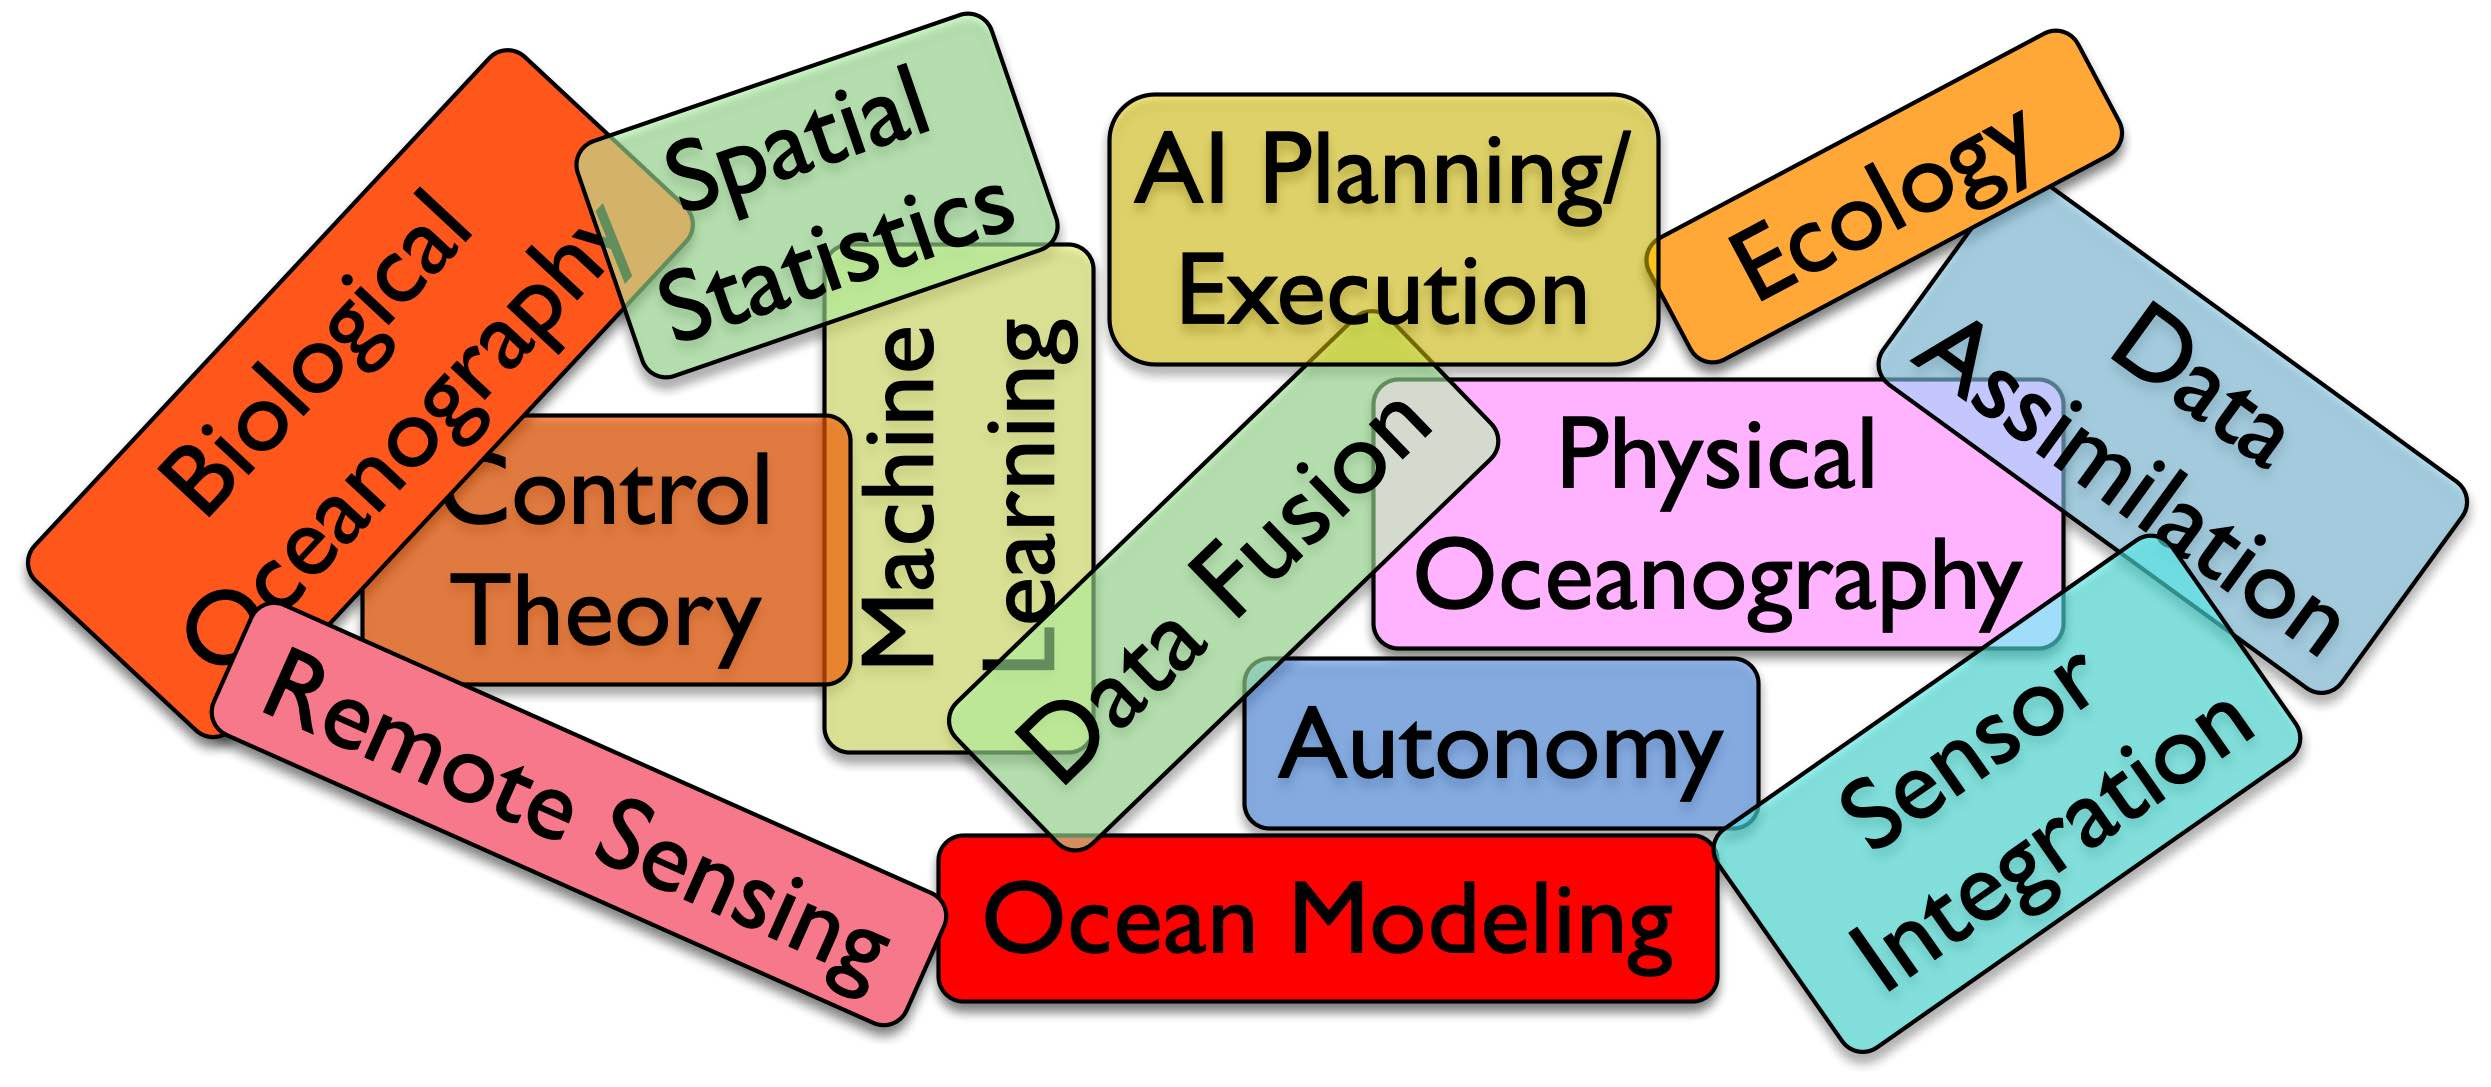
\includegraphics[scale=0.08]{fig/concepts.jpg}
  \caption{\proj is highly interdisciplinary across a range of
    engineering and scientific disciplines.}
  \label{fig:concepts}
\end{wrapfigure}

\noindent
The \proj team is highly inter-disciplinary and includes members from
diverse backgrounds including biological and physical oceanography,
modeling, Artificial Intelligence decision making, Robotics, Control
Theory and Operational Oceanography (Fig. \ref{fig:concepts}). The
members of the team have known each other for some time and in many
instances have worked together for more than a decade.  The proposed
effort is \emph{integrative}, in that work in these diverse fields has
advanced in siloed environments or in other domains -- with \proj we
plan to bring together the disparate elements in ways hitherto not
done before, especially the tight integration of AI-driven marine
robotic vehicles in the aerial, surface and underwater domains with
modeling and control. In doing so, integration between model
prediction and assimilation will be enhanced so as to provide
realistic forecasts of a range of biophysical variables including
temperature, salinity, wind, surface and subsurface currents and
bio-optical properties. These in turn will be used to intelligently
target sampling with these multi-domain platforms. Important outcomes
of this proposed project include:

\begin{itemize}

\item rapid assessment of environmental state using state of the art
  methods in modeling, control and sampling with minimal human
  intervention
  
\item increasing model prediction skill with targeted sampling to reduce
  uncertainty
  
\item real-time decision support to determine appropriate mix of robotic
  or manned assets (e.g. small boats or research vessel) for targeted
  sampling
  
\item demonstration of coordinated observations with an ensemble of
  robotic vehicles with minimal human intervention

\item outreach to local communities to demonstrate advanced
  capabilities in prediction and forecasting ocean conditions

\end{itemize}  

The novelty of this proposed effort is in the integrative aspects of a
field exercise; while individual aspects might have been demonstrated
in other field experiments (including by members of this team), \proj
will leap-frog experimental design, autonomous operations,
assimilation, modeling and prediction in ways not done before.

